\documentclass[11pt]{article}

\usepackage{a4wide}
\usepackage[utf8]{inputenc}
\usepackage[russian]{babel}
\usepackage{graphicx}
\usepackage{amsmath}
\usepackage{amsthm}
\usepackage{amssymb}
\usepackage{url}

\newtheorem{ConvexHull}{Определение}

\newcommand*{\hm}[1]{#1\nobreak\discretionary{}{\hbox{$\mathsurround=0pt #1$}}{}}
\newcommand\abs[1]{\left\lvert#1\right\rvert}
\newcommand{\scalar}[2]{\left<#1,#2\right>}
\newcommand\norm[1]{\left\lVert#1\right\rVert}

\DeclareMathOperator{\conv}{Conv}

\begin{document}
\thispagestyle{empty}

\begin{center}
\ \vspace{0cm} % WTF?! There were -3cm in example, but it worked strange.
\includegraphics[width=0.5\textwidth]{msu.eps}\\
{\scshape Московский государственный университет имени М.~В.~Ломоносова}\\
Факультет вычислительной математики и кибернетики\\
Кафедра системного анализа

\vfill
{\LARGE Отчёт по практикуму} \\
\vspace{1cm}
{\Huge\bfseries <<Решение краевой задачи для уравнения теплопроводности на сегменте методом Фурье>>}
\end{center}

\vspace{1cm}
\begin{flushright}
\large
\textit{Студент 315 группы}\\
В.~С.~Терёшин\\
%\vspace{5mm}
%\textit{Руководитель практикума}\\
%к.ф.-м.н., доцент П.~П.~Петров
\end{flushright}

\vfill
\begin{center}
Москва, 2013
\end{center}

\pagebreak

\section{Постановка задачи}
Имеется дифференциальное уравнения в частных производных с граничными условиями, описывающее процессы теплопроводности в тонком металлическом стержне:
$$
\left\{
\begin{aligned}
u_t = a^2u_{xx} \\
t \in [0, T], x \in [0, l] \\
u(0, t) = 0 \\ u(l, t) = 0 \\
u(x, 0) = \varphi(x).
\end{aligned}
\right.
$$
Решением данной краевой задачи называется функция $u(x, t)$, удовлетворяющая следующим требованиям:
\begin{enumerate}
\item
$u(x, t)$ определена и непрерывна в замкнутой области $0 \leqslant x \leqslant l, \; 0 \leqslant t \leqslant T$.
\item
$u(x, t)$ удовлетворяет уравненю теплопроводности в открытой области $0 \hm< x \hm< l, \; 0 \hm< t \hm< T$.
\item
$u(x, t)$ удовлетворяет начальному и граничному условиям, т.~е. $u(x, 0) = \varphi(x), \; u(0, t) \hm= u(l, t) \hm= 0$.
\end{enumerate}
Необходимо решить это уравнение методом Фурье. Кроме этого, необходимо реализовать решение таких уравнений для любых $\varphi$,
$a$, $l$ и при ограничении $0 < t < T$ на языке \texttt{Matlab}.

\section{Аналитическое решение}
Будем решать данную задачу методом разделения переменных (методом Фурье).

Будем искать решение в виде $u(x, t) = X(x)T(t)$. Подставляя это представление $u$ в исходное уравнение, получаем:
$$
X(x)T'(t) = a^2X''(x)T(t).
$$
Разделим выражение на $a^2X(x)T(t)$:
$$
\frac{1}{a^2} \frac{T'(t)}{T(t)} = \frac{X''(x)}{X(x)} = -\lambda, \; \lambda = \mathrm{const}.
$$
Так как в левой части уравнения у нас находится функция зависящая только от $t$, а в правой --- только от $x$, то, фиксируя любое значение $x$ в правой части, получаем, что для любого $t$ значение левой части уравнения постоянно. Таким же образом можно убедиться, что и правая часть постоянна, то есть равна некой константе $-\lambda$ (минус взят для удобства). Таким образом, мы получаем два обыкновенных линейных дифференциальных уравнения:
\begin{gather}
X''(x) + \lambda X(x) = 0, \notag \\
T'(t) + a^2 \lambda T(t) = 0. \notag
\end{gather}
Обратим внимание на граничные условия исходной задачи и подставим в них предполагаемый вид уравнения, получим:
$$
\left\{
\begin{aligned}
u(0, t) = X(0)T(t) = 0 \\
u(l, t) = X(l)T(t) = 0,
\end{aligned}
\right.
$$
откуда $X(0) = X(l) = 0$ (иначе $T(t) \equiv 0$, откуда $u(x, t) = 0$, а мы ищем только нетривиальные решения).

С учетом полученных граничных условий мы получаем задачу Штурма--Лиувилля:
$$
\left\{
\begin{aligned}
X''(x) + \lambda X(x) = 0 \\
X(0) = X(l) = 0.
\end{aligned}
\right.
$$
Её решение сводится к решению линейного дифференциального уравнения и рассмотрению трёх случаев:
\begin{enumerate}
\item
$\lambda < 0$.

В этом случае общий вид решения будет следующим:
$$
X(x) = C_1 e^{\sqrt{-\lambda}x} + C_2 e^{-\sqrt{-\lambda}x}.
$$
Подставив граничные условия, мы убедимся, что решение будет $X(x)\equiv 0$, а мы ищем только нетривиальные решения, следовательно, этот случай не подходит.

\item
$\lambda = 0$.

Общий вид решения
$$
X(x) = C_1 x + C_2.
$$
Несложно убедиться, что этот вариант нам также не подходит.

\item
$\lambda > 0$.

Общий вид решения
$$
X(x) = C_1 \cos(\sqrt\lambda x) + C_2 \sin(\sqrt\lambda x).
$$
Подставим граничные условия:
\begin{gather}
X(0) = C_1 = 0, \notag \\
X(l) = C_2 \sin(\sqrt\lambda l) = 0. \notag
\end{gather}
Так как мы ищем только нетривиальные решения, $C_2 = 0$ нам не подходит, следовательно
\begin{gather}
\sin(\sqrt\lambda l) = 0, \notag \\
\sqrt\lambda l = \pi k, \quad k = 1, \; 2, \; \ldots \notag \\
\lambda_k = \left(\dfrac{\pi k}{l}\right)^2,\quad k = 1, \; 2, \; \ldots \notag
\end{gather}
Отсюда
$$
X_k(x)=C_k\sin\left(\dfrac{\pi k}{l} x \right),\;\quad k = 1, \; 2, \; \ldots
$$
\end{enumerate}

C учетом найденных $\lambda$, найдём общее решение линейного дифференциального уравнения
$$
T'(t) + a^2 \left(\dfrac{\pi k}{l}\right)^2 T(t)=0.
$$
Получим ответ:
$$
T_k(t)=C_k \exp\left( -a^2\left(\dfrac{\pi k}{l}\right)^2 t \right), \quad C_k = \mathrm{const}.
$$

Теперь решение исходной задачи:
\begin{gather}
u_k(x, t) = X_k(x) T_k(t) = C_k \sin\left( \sqrt{\lambda_k} x \right) e^{-a^2 \lambda_k t}, \quad k = 1, \; 2, \; \ldots \notag \\
u_k(x, t) = X_k(x) T_k(t) = C_k \sin\left(\frac{\pi k}{l} x \right) \exp\left(-a^2\left(\dfrac{\pi k}{l} \right)^2 t \right),\quad k = 1, \; 2, \; \ldots \notag
\end{gather}

В результате у нас получилось бесконечное количество частных решений уравнения. Все эти частные решения линейно независимы, то есть линейная комбинация любого количества решений равна нулю, только если все коэффициенты при них равны нулю. Поэтому суммируя все частные решения по $n$ от единицы до бесконечности, мы получим общее решение исходной задачи:
$$
u(x, t) = \sum\limits_{k=1}^\infty u_k(x, t) = \sum\limits_{k=1}^\infty C_k \sin\left( \sqrt{\lambda_k} x \right) e^{-a^2 \lambda_k t}.
$$

Осталось определить значения $C_k$ из начального условия $u(x,0) \hm= \varphi(x)$.
Для того, чтобы определить значение $C_k$, необходимо разложить функцию $\varphi(x)$ в ряд Фурье:
\begin{gather}
\varphi(x) = \sum\limits_{k=1}^\infty A_k\sin\left(\dfrac{\pi k}{l}x\right), \notag \\ 
A_k = \frac{2}{l} \int\limits_0^l \varphi(\xi) \sin\left(\dfrac{\pi k}{l} \xi \right)\, d\xi. \notag
\end{gather}
Получаем:
\begin{gather}
u(x, 0) = \sum\limits_{k=1}^\infty C_k\sin\left( \dfrac{\pi k}{l} x \right) = \sum\limits_{k=1}^\infty A_k\sin\left(\dfrac{\pi k}{l} x\right), \notag \\
C_k = A_k = \frac{2}{l} \int\limits_0^l \varphi(\xi) \sin\left(\dfrac{\pi k}{l}\xi\right)\, d\xi. \notag
\end{gather}

Откуда общее решение:
$$
u(x, t) = \sum\limits_{k=1}^\infty \left(\dfrac{2}{l} \int\limits_0^l \varphi(\xi) \sin\left(\dfrac{\pi k}{l}\xi\right)\, d\xi\right) \sin\left(\dfrac{\pi k}{l}x\right)\exp\left(-a^2\left(\dfrac{\pi k}{l}\right)^2 t\right).
$$

В курсе математической физики доказывается, что полученный ряд удовлетворяет всем условиям данной задачи, то есть функция $u(x, t)$ дифференцируема (и ряд сходится равномерно), удовлетворяет уравнению в области определения и непрерывна в точках границы этой области.

\section{Формат входных и выходных данных}
Реализовання функция \texttt{fourier\_solver} принимает следующие параметры:
\begin{enumerate}
\item
\texttt{phi} --- \texttt{function handler} на функцию $\varphi$ из постановки задачи.
\item
\texttt{a} --- константа $a$ из постановки задачи.
\item
\texttt{l} --- правая граница рассматриваемого в задаче отрезка.
\item
\texttt{T} --- время, до которого необходимо получить решение.
\item
\texttt{k} --- количество вычисляемых членов рядов.
\item
\texttt{dl} --- расстояние между точками, в которых ищется решение.
\item
\texttt{dT} --- промежутки времени, через которорые ищется решение.
\end{enumerate}

Функция \texttt{fourier\_solver} возвращает матрицу размером $n \times m$, в которой в строке $i$ и столбце $j$ стоит $u((i - 1) \delta l, (j - 1) \delta T)$, $n$ и $m$ такие что $(n - 1) \delta l \leqslant l$ и $(m - 1) \delta T \leqslant T$.

\section{Примеры работы}
\begin{enumerate}
\item
$$
\left\{
\begin{aligned}
u_t = u_{xx}, \; t \in [0, 5], \; x \in [0, 1] \\
u(0, t) = u(l, t) = 0 \\
u(x, 0) = 2.9 \sin(\pi x) + 4.8 \sin(3 \pi x) \\
k = 10, \; \delta l = 0.01, \; \delta T = 0.001.
\end{aligned}
\right.
$$
Здесь и далее $k$ --- количество членов для суммирования, $\delta l$ и $\delta T$ - промежутки вычисления значения функции по расстоянию и по времени соответственно.

\includegraphics[scale=0.8]{image1.eps} \newline
\item
$$
\left\{
\begin{aligned}
u_t = u_{xx}, \; t \in [0, 5], \; x \in [0, 2.1254] \\
u(0, t) = u(l, t) = 0 \\
u(x, 0) = -2x (2x - 2) (2x - 3) (2x - 4) + 3 \\
k = 100, \; \delta l = 0.01, \; \delta T = 0.001.
\end{aligned}
\right.
$$

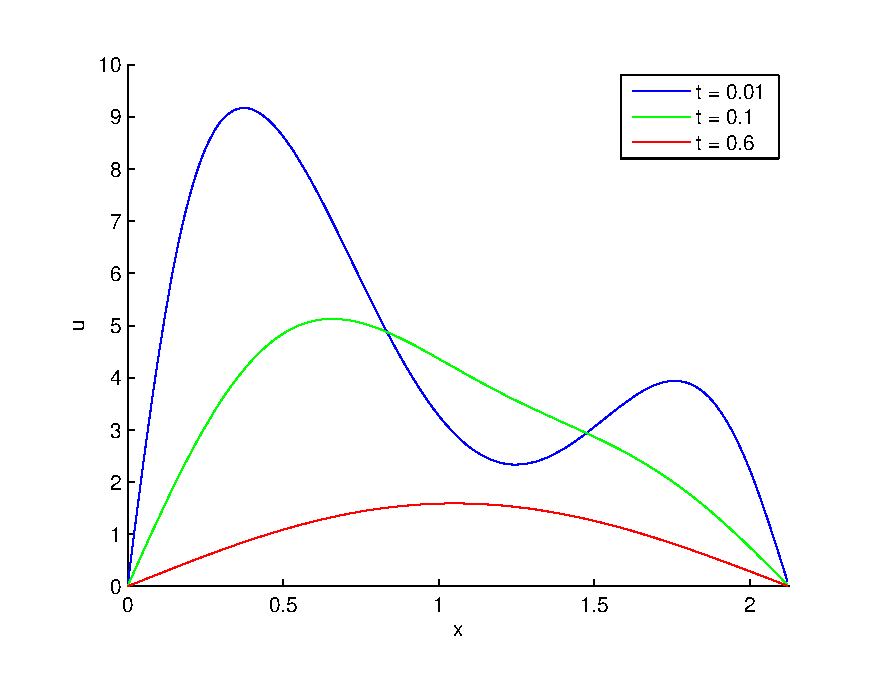
\includegraphics[scale=0.8]{image2.eps} \newline
\item
$$
\left\{
\begin{aligned}
u_t = u_{xx}, \; t \in [0, 5], \; x \in [0, \pi] \\
u(0, t) = u(l, t) = 0 \\
u(x, 0) = \cos^2(x - \dfrac{\pi}{2}) \\
k = 100, \; \delta l = 0.01, \; \delta T = 0.001.
\end{aligned}
\right.
$$

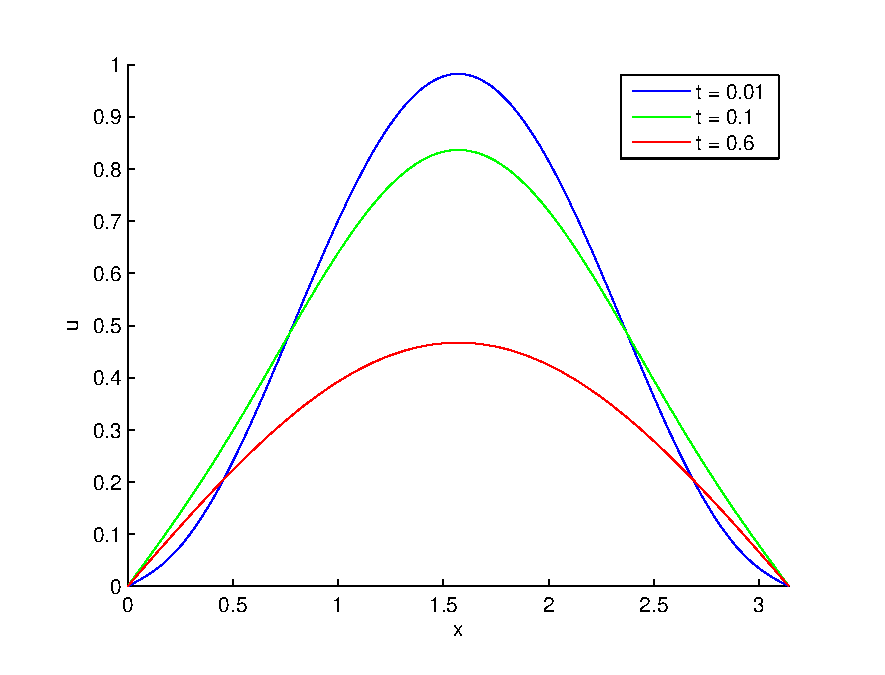
\includegraphics[scale=0.8]{image3.eps} \newline
\end{enumerate}

\Работа{Пример с точным аналитическим решением}
section требуемой функции сравнивалась с известным точным решением следующей системы:
$$
\left\{
\begin{aligned}
u_t = 0.4u_{xx}, \; t \in [0, 5], \; x \in [0, 1] \\
u(0, t) = u(l, t) = 0 \\
u(x, 0) = 2.9 \sin(\pi x) + 4.8 \sin(3 \pi x) \\
k = 10, \; \delta l = 0.01, \; \delta T = 0.001.
\end{aligned}
\right.
$$

$ u(x, y) = 2.9 e^{-0.4 \pi^2 t} \sin(\pi x) + 4.8 e^{-3.6 \pi^2 t} \sin(3 \pi x) $ --- точное решение, а $V$ --- матрица численного решения с помощью нашей функции.

Рассмотрим матрицу $A$, где $A_{ij} = V_{ij} - u((i - 1) \delta l, (j - 1) \delta T)$.

$\norm{A} = 2.8606 \cdot 10^{-14}$, что означает, что реализованное решение в системе \texttt{Matlab} в выбранных точках отличается от точного решения на достаточно малую величину, что означает корректность работы реализованной фукнции на этих входных данных.

\begin{thebibliography}{99}
	\bibitem{Wiki} \url{http://en.wikipedia.org/wiki/Heat_equation}
	\bibitem{Tihonov} А.~Н.~Тихонов, А.~А.~Самарский. Уравнения математической физики. М.:~Изд-во МГУ, 1999.
	\bibitem{Zaharov} Е.~В.~Захаров, И.~Н.~Дмитриева, С.~И.~Орлик. Уравнения математической физики. Методическое пособие. М.:~Издательский отдел Факультета ВМиК МГУ им.~М.~В.~Ломоносова, 2005.
	\bibitem{IAD} Дигайлова~И.~А. Лекции по \LaTeX. 2009.
\end{thebibliography}
\end{document}
